\documentclass[prl, twocolumn]{revtex4-1}

\usepackage{graphicx}
\usepackage{color}
\usepackage{latexsym,amsmath}
%\usepackage{booktabs}
\usepackage[utf8]{inputenc}
\usepackage{array}
\usepackage{wrapfig}
\usepackage{multirow}
\usepackage{tabularx}

\definecolor{linkcolor}{rgb}{0,0,0.65} %hyperlink
\usepackage[pdftex,colorlinks=true, pdfstartview=FitV, linkcolor= linkcolor, citecolor= linkcolor, urlcolor= linkcolor, hyperindex=true,hyperfigures=true]{hyperref} %hyperlink%

\begin{document}

\title{MaFalDDa -- Convolutional NN for analyzing time series}

\author{Delfina Iriarte}
\author{Davide Maniscalco}
\author{Mattia Pujatti}
\author{Fabio Semenzato}
\date{\today}

\begin{abstract}
  The purpose of this work is studying several aspects of the training with convolutional neural networks, used in this case to analyze time series. Data are generated sampling an exponential distribution, and then a pattern in the data is introduced using a sine function. Some convolutional neural networks are built and their performances tested, with the constraint of having less than 600 parameters. Finally, also the impact of the regularization is studied, together with new different data, generated with a different signal-to-noise ratio.
\end{abstract}

\maketitle
\section{Introduction}

Convolutional Neural Networks (CNN) gained considerable interest during the past years both in the field of speech and image analysis. One of the main features is that the model complexity and the number of weights is efficiently reduced by \textit{weight sharing} and restriction to local connections. Moreover, a convolutional neural network can be described as a translationally invariant neural network that respects locality of the input data \cite{Metha}. \

Within a convolutional architecture, there are several possibilities for combining different kind of layers and learning rules. A typical architecture of a CNN is shown in Figure \ref{fig:fig1}, on the right, and it is formed by Convolutional layers, Pooling layers, and Fully-Connected Layers. 

\begin{figure*}[!tb]
    \centering
    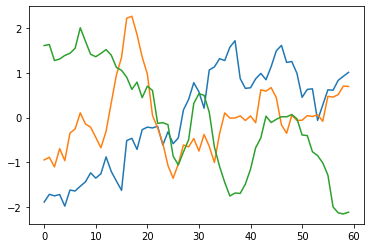
\includegraphics[width=0.3\textwidth]{pics/data_ex.png}
    \hspace{1cm}
    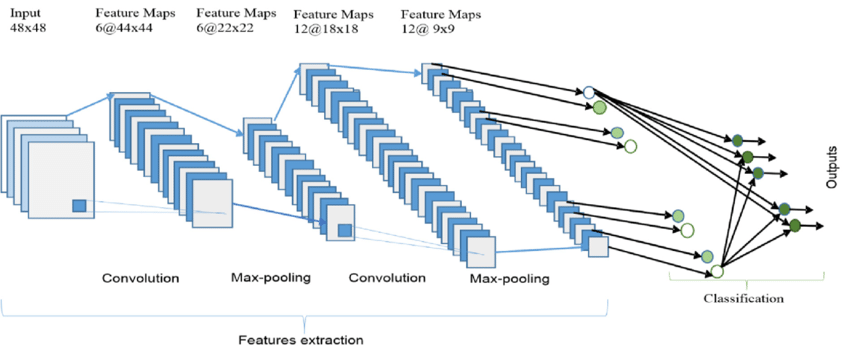
\includegraphics[width=0.6\textwidth]{pics/figure1.png}
    \caption{\textit{Left}: in orange, green and blue are represented three data samples. \textit{Right}: example of architecture of a convolutional neural networks with their typical layers.}
    \label{fig:fig1}
\end{figure*}


The purpose of this paper is to study the several hyper-parameters of a CNN, using as a dataset a diffusive time series, and to compare the performances of different models proposed. 

\section{Methods}

\subsubsection{Data Generation}
The data consist of time-series samples. Each sample is composed of 60 time steps and each time step is linked to the one before as $y_i = y_{i-1} + dy + b$, where $dy$ is a random noise, which amplitude is controlled and independent from the value of $y$, and $b$ is a constant bias, which causes the sample to have an overall positive slope; the first time step refers to the last time step of the previous sample. Then, to each of these samples thus generated, we added one of these 3 signals, each one with probability 1/3:
\begin{itemize}
    \item \textit{Zero Signal}: the sample has been left unchanged; we will assign them to Label 0;
    \item \textit{Positive Signal}: we added, at a random position inside the sample, the positive phase of a sinusoid, with constant period and amplitude; we will assign them to Label 1;
    \item \textit{Negative Signal}: we added, at a random position inside the sample, the negative phase of a sinusoid, with the same period and amplitude of the positive one; we will assign them to Label 2.
\end{itemize}

An example of data analyzed is given in figure \ref{fig:fig1} left (the data shown are already prepared as explained in the section \textit{Results}). Recall that this is a supervised learning problem.

\subsubsection{Data Preparation}

Since there is a constant additive bias at each time step, the magnitude of the values keep increasing from sample to sample. This would make it almost impossible for the neural network to detect the patterns, since the high variance of the inputs would make the optimization really unstable. Therefore, we had to subtract the mean out of each sample. Moreover, a trend inside the sample would slower the training as well, thus, we subtracted from the n-th time step the mean of the n-th time steps of all the samples.

\subsubsection{Search for the best model}



In the search for the best model, various points have been taken into account:

\begin{itemize}
    \item \textbf{Restrictions}: for this project, we have been asked to provide the best architecture with a number of trainable parameters less than 600.
    \item \textbf{Initializer}: a random normal initializer was used in the beginning, however we noticed that switching to the He normal initializer improved the training speed.
    \item \textbf{Data Augmentation}: beside the restriction on the number of parameters of our model, another limiting one has been the small number of training sample. In order to solve this, we opted for a Gaussian-Noise Layer as the initial layer, which would act on the input before passing it to the convolutional layer.
    \item \textbf{Convolutional Layers}: the kernel size of the first convolutional layer should be large enough to include the half-period of the sinusoid. Moreover, the number of filters should be at least 2, in order to detect the positive and negative phases of the sinusoid (the Zero Signal could be detected by a low activation of these two filters).
    \item \textbf{Pooling Layers}: the number of pooling layers, as well as their pooling size, highly influence the number of parameters of the convolutional part, as well as the number of connections with the fully connected part. Thus, they have been useful in order to control the number of total parameter and to restrict it to be less than 600. As regarding the type of pooling layer, both the Average Pooling and the Max Pooling have been tried.
    \item \textbf{Activation Function}: the activation functions we tried are: ELU, ReLU and PReLU. The problem with the PReLU is that, by default, it trains a different slope for every neuron of the layer, thus increasing a lot the number of trainable parameters. However, it is possible to share a single slope among various neurons, in order to reduce the number of additive trainable parameters.
    \item \textbf{Regularization}: we needed to introduce some regularization in order to make the training more stable and to avoid overfitting. Thus, we added dropout layers between the fully-connected ones and a weight regularizer that we chose between l1, l2 and a mixture of these two.
\end{itemize}

\vspace{-.2cm}

\section{Results}

\subsubsection{Best Model Found}

After an extensive search of the optimal architecture and a fine tuning of the hyperparameters, the best model found is the following:

\begin{table}[h]
\begin{tabular}{p{7cm}}
    \textbf{Gaussian Noise Layer}, with standard deviation $0.07$ \\
    \vspace{0pt}
    \textbf{Convolutional Layer}, with 7 filters, kernel size of $15$ and a $l2$ regularization with $\lambda=0.01$ \\
    \vspace{0pt}
    \textbf{PReLU Activation Function}, with a different trainable slope for each convolutional filter \\
    \vspace{0pt}
    \textbf{Max Pooling}, with pooling size 6 and a padding copying the first time step to the left and last time step to the right \\
    \vspace{0pt}
    \textbf{Convolutional Layer}, with 6 filters, kernel size of 3 and a $l2$ regularization with $\lambda=8\cdot10^{-5}$ \\
    \vspace{0pt}
    \textbf{PReLU Activation Function}, with a different trainable slope for each convolutional filter \\
    \vspace{0pt}
    \textbf{Dense Layer}, with 8 neurons and a $l2$ regularization with $\lambda=8\cdot10^{-5}$ \\
    \vspace{0pt}
    \textbf{Dropout Layer}, with probability 0.16 \\
    \vspace{0pt}
    \textbf{Dense Layer}, with 3 neurons and softmax activation function, which output corresponds to the probability of belonging to each of the 3 labels \\
\end{tabular}
\end{table}

In Table \ref{tab:best_model} we report a brief summary of the best model along with the trainable parameters of each layer.

\begin{table}[!tb]
\begin{tabular}{c c}
    \toprule
    Layer (type) & Trainable Parameters\\\colrule
    Gaussian Noise & 0\\
    Convolutional & 112\\
    PReLU & 7\\
    Max Pooling & 0\\
    Convolutional & 132\\
    PReLU & 6\\
    Flatten & 0\\
    Dense & 296\\
    Dropout & 0\\
    PReLU & 1\\
    Dense & 27\\
    \colrule
    Total & 581 \\
    \botrule
\end{tabular}
\caption{Summary of the best model along with the trainable parameters.}
\label{tab:best_model}
\end{table}

\begin{figure*}[!tb]
    \centering
    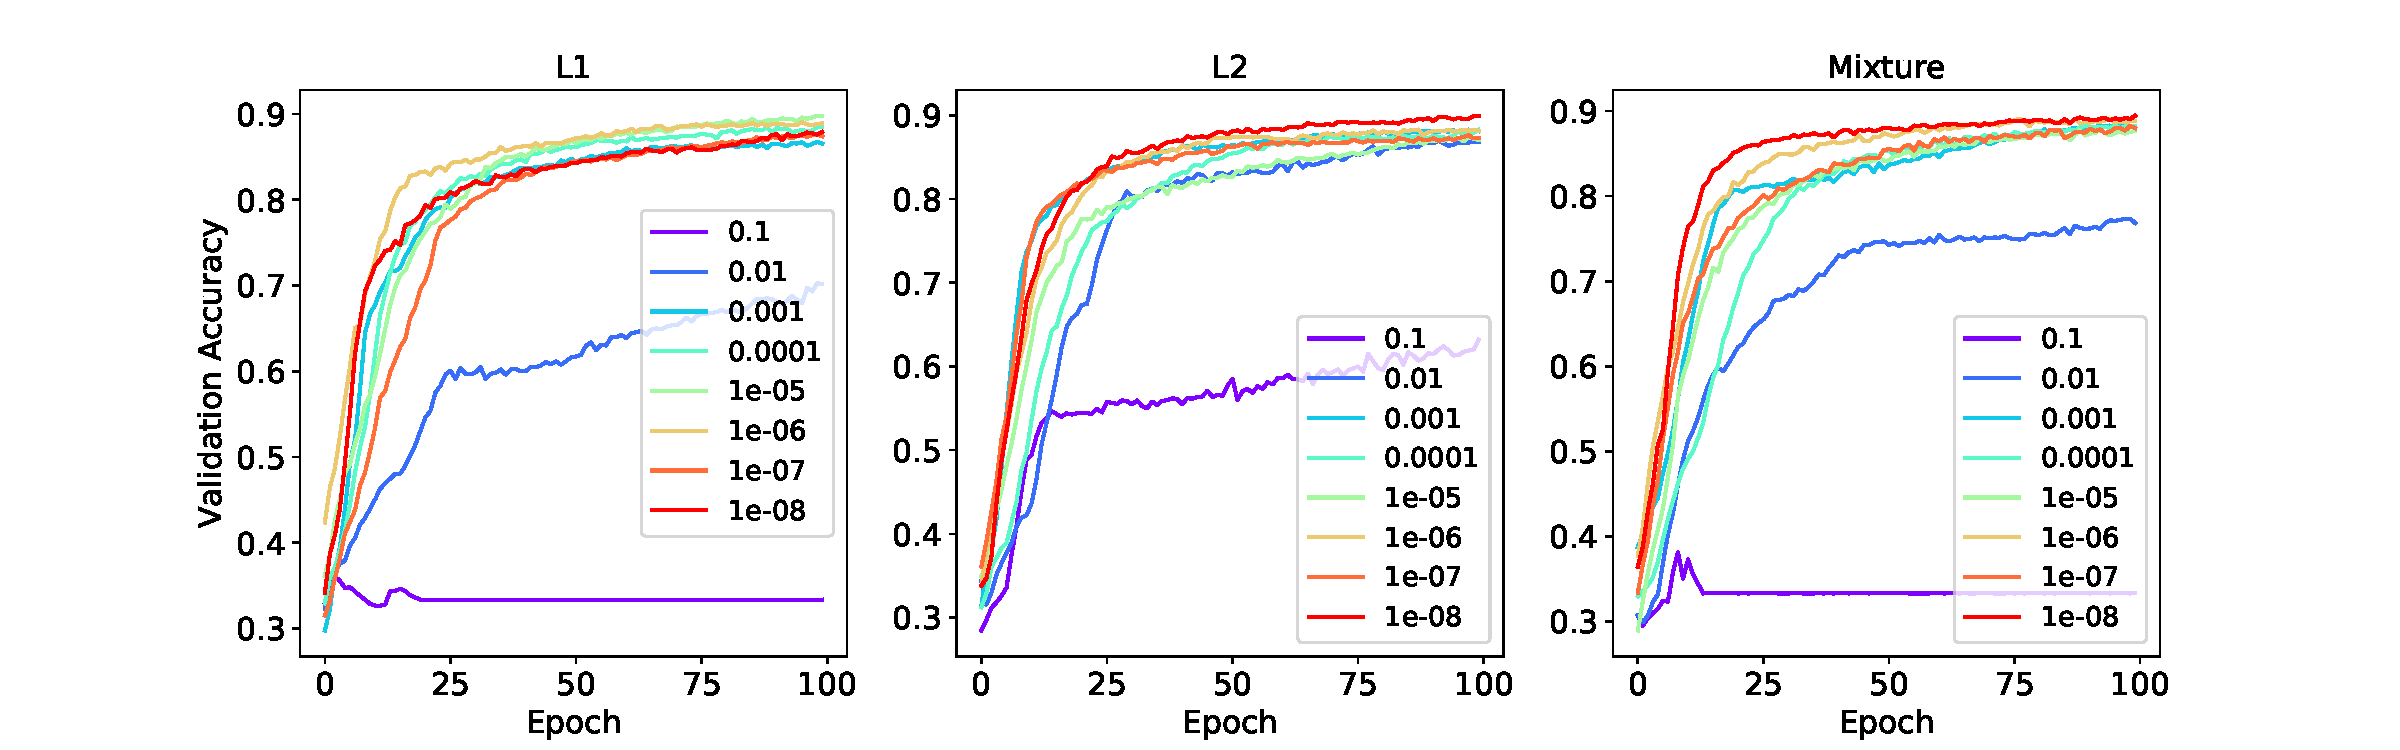
\includegraphics[width=1.05\textwidth]{pics/regularization.pdf}
    \caption{Accuracy over the validation set for the regularization (a)\textit{l1}, (b) \textit{l2}, (c) \textit{l1\_l2}; the values reported in the plots represent the weight of the regularization in the loss function.}
    \label{fig:val_acc_l1}
\end{figure*}

\begin{figure}[!tb]
    \centering
    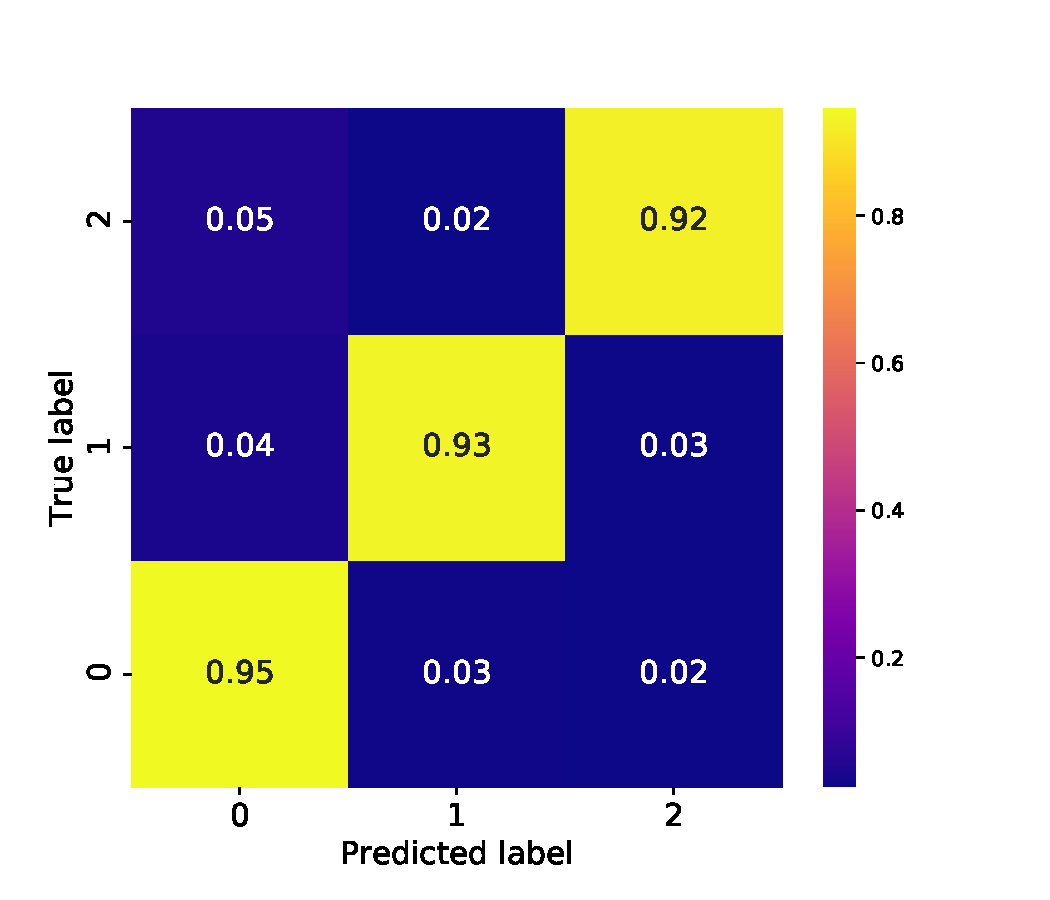
\includegraphics[width=0.38\textwidth]{pics/norm_conf_mat.pdf}
    \caption{Normalized confusion matrix on the validation set for the best model.}
    \label{fig:confusion_matrix}
\end{figure}

\subsubsection{Confusion Matrix}

We report in Figure \ref{fig:confusion_matrix} the confusion matrix of the best model found. We can see that all the 3 classes are well separated and there are no strong cases of confusion between two classes. As predictable, the class which has the highest TPR (True Positive Rate) is the \textit{Zero Signal} one, since it does not require a structured convolutional filter to be detected.



\subsubsection{Analysis of regularization}

In Figure \ref{fig:val_acc_l1} we report the training evolution of the validation accuracy, using various regularizations for our model. As explained in Section \textit{Methods}, we tried three different regularization losses: \textit{l1}, called \textit{Lasso Regression}, \textit{l2}, called \textit{Ridge Regression}, and a symmetric mixture of these two. The values reported in the plots represent the weight of the regularization in the loss function. We can notice that the model seems to perform better with smaller regularizations; moreover, with high regularizations the training starts to fail. It is possible to see that the \textit{l1} method seems to have a slower convergence, while the \textit{l1\_l2} seems to convergence faster but is more unstable. Thus, we chose as optimal method the \textit{l2} one.



\subsubsection{Test on different data}

Finally, we wanted to study the performance of our model on data with different signal-to-noise ratio, meaning in modifying the amplitude of the sinusoid for the Positive and Negative Signal classes. We report our results in Figure \ref{fig:point4_acc}. It is possible to notice a systematic decreasing of the accuracy as the amplitude decreases; the training starts to fail for amplitudes that are half the original one, while the accuracy tends to 1 quickly as we increase the original amplitude.

\begin{figure}[h]
    \centering
    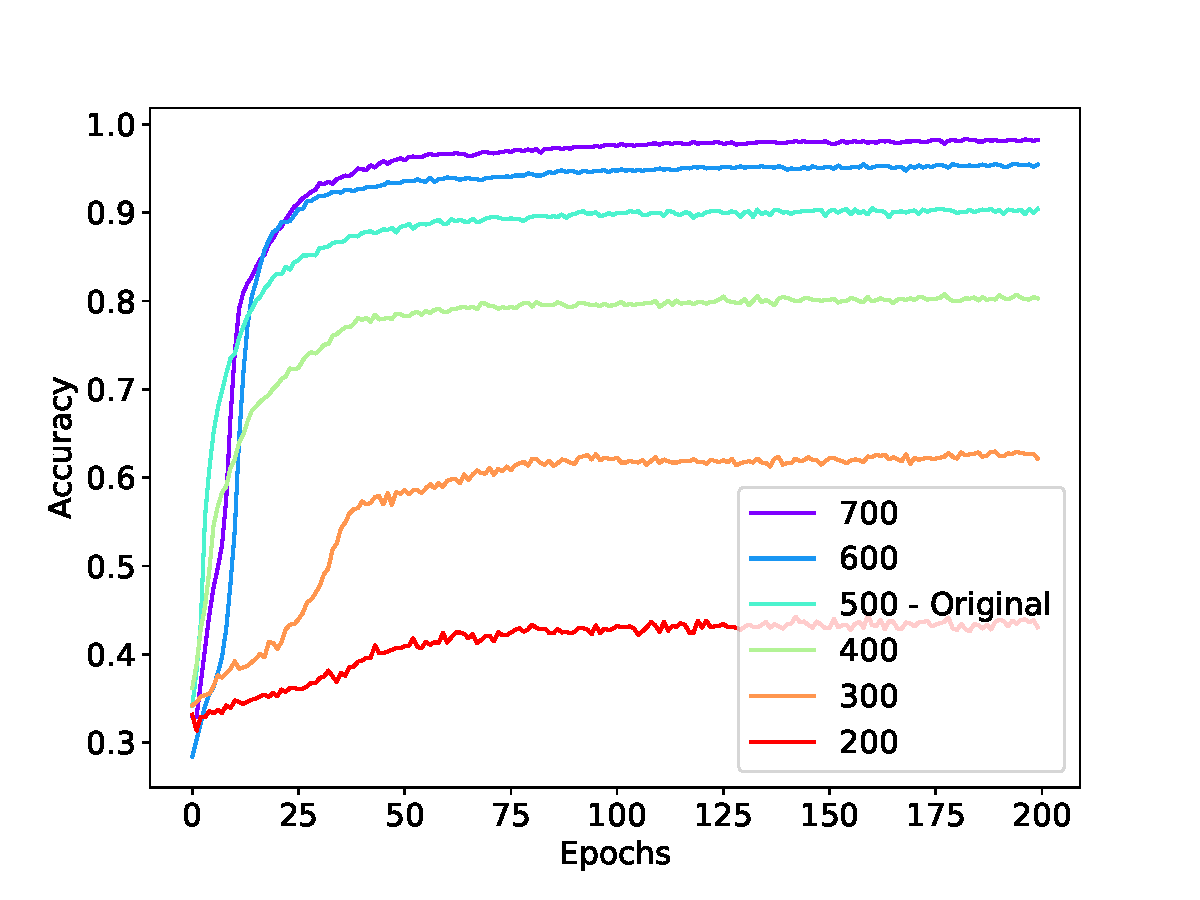
\includegraphics[width=0.42\textwidth]{pics/sig_noise.pdf}
    \caption{Accuracy over the validation set, varying the amplitude of the signal.}
    \label{fig:point4_acc}
\end{figure}


\section{Conclusions}

This project highlighted some key points that are needed to be taken into account when facing particular tasks, which require the features extraction power of the Convolutional Neural Networks. We went through the most important layers needed to build this kind of architecture, as well as the main hyperparameters that are needed to be tuned in order to reach a better and faster convergence.

Moreover, we quickly discussed how to deal with a restriction on the total number of trainable parameters. This could be useful in real-world applications when deeper and wider Convolutional Neural Networks are needed to analyze more complex samples: lowering the number of trainable parameters improves the training speed and decreases the risk of overfitting. We showed as well three different regularization methods, useful to further decrease this risk.


\begin{thebibliography}{99}

\bibitem{Metha}
  P. Metha et al.,
  "A high-bias, low-variance introduction to Machine Learning for physicists", Physics reports
  {\bf 810}, 61-63 (2019)
  
\end{thebibliography}

\end{document}
